% 黒魔術
\expandafter\ifx\csname ifdraft\endcsname\relax
    \documentclass[a4paper,twoside,12pt,papersize, dvipdfmx]{iirthesis}
    \usepackage{amsmath,amssymb,amsthm}
    \usepackage{graphicx}
    \usepackage{subcaption}
    \usepackage{url}
    \usepackage{otf}
    \usepackage{minitoc}
    \usepackage{bm}
    \usepackage{amsmath,amssymb}
    \usepackage{times} % times new roman
    \begin{document}
    % ベンリダナー
    \newcommand{\figref}[1]{\figurename\ref{#1}}
    \newcommand{\tabref}[1]{\tablename\ref{#1}}
    \renewcommand{\eqref}[1]{式~(\ref{#1})}
    \newcommand{\chapref}[1]{\ref{#1}章}
    \newcommand{\secref}[1]{\ref{#1}節}
    \newcommand{\ssecref}[1]{\ref{#1}項}
    \newcommand{\appref}[1]{付録\ref{#1}}
\fi


\chapter{結論}\label{chap::conclusion}
\minitoc
\section{結論}\label{sec::conclusion::conclusion}
本研究では,センサレスin-handケージングマニピュレーションの有用性を高め,パーツフィーダを実用化するために,新たなハンド構成である対向型ハンドの提案,動作計画の計算時間と位置決め精度の総合的な性能向上の2つについて取り組んだ.前者に関して,従来のハンド構成,並列型ハンドではマニピュレーションの際,ジャミングという問題が発生していた.これに対して従来研究において様々な解決法が試みられたが,依然として一定の頻度でジャミングは発生していた.また,並列型ハンドの根元付近は構造上マニピュレーションできないという問題があった.そこで,対向型ハンドの提案により,ジャミングを限りなく減らすことができ,またどこに対象物があってもマニピュレーションできるようになった.後者に関しては,まず従来法である順探索アルゴリズムの改善を行った.パーツフィーダへ応用を考慮した探索終了条件の緩和,$\mathcal{C}_{\mathrm{free\_obj}}$の効率的な抽出により計算時間を大幅に削減した.また,動作計画より得られた最終姿勢からハンドを対象物に向けて狭めていくという手法により,位置決め精度も向上させた.次に,逆探索アルゴリズムを提案した.マニピュレーション終了時の位置決めされたハンド姿勢を探索の初期値としてユーザーが与える(,または最適姿勢生成アルゴリズムによって生成する)ことができるため,位置決め精度の高い経路が生成されることが保証されている.最後に両側探索アルゴリズムを提案した.順探索アルゴリズムと逆探索アルゴリズムを組み合わせたアルゴリズムであり,マニピュレーション開始姿勢から終了姿勢へ,またその逆への非常に強いバイアスがかかるため効率の良い探索アルゴリズムとなっている.実際に計算時間の短縮が確認できた.また,順探索アルゴリズム,逆探索アルゴリズムの両方の位置決め精度向上の仕組みも引き継いでいるため,位置決め精度も同様に高くなっている.これら3つのアルゴリズムの中では,両側探索アルゴリズムが計算時間,位置決め精度の面で最も優れているが,ユーザーのニーズによっては他の探索アルゴリズムが適している場合もあり,各々使い分けられるというのも本手法の有用性を高めている.\par

本動作計画で生成した経路を用いて,長方形,三角形,L字型,T字型物体に対して実機でマニピュレーションを行った.ロボットハンドには,3リンク3関節のハンドを向かい合うように2つ組み合わせた対向型ハンドを用いた.結果,いずれの対象物においても,ジャミングなく目標位置・姿勢までマニピュレーションされることを確認した.しかし,実機の誤差により計算程の位置決め精度は得られなかった.

以上,対向型ハンドの提案,動作計画の高性能化によりセンサレスin-handケージングマニピュレーションの有用性を高めることができた.これにより,ジャミングが起こらず安定し,かつ再立ち上げ時間が短く,位置決め精度が高い汎用パーツフィーダの実用化に貢献できたと考えている.

\section{今後の展望}\label{sec::conclusion::future}
\subsection*{マニピュレーションタスクの汎用性}
現状,一部の限られた位置・姿勢の対象物しか,目標位置・姿勢へとマニピュレーションできないという問題がある.L字形物体で考えると,目標位置・姿勢からおよそ$\pm 45^\circ$の姿勢の対象物しか取り扱えず,例えば下向きの$\phi=180^\circ$のL字形物体を上向きの$\phi=0^\circ$の状態へ反転させるような動作経路を生成するのは困難である.本研究では,センサレスであるため対象物の位置・姿勢に関わらず同じハンド動作で同じ目標位置・姿勢へ運べるようなハンド動作を計画している.おそらく上記の例のような反転させるマニピュレーションと既に目標位置・姿勢付近であり微調整するようなマニピュレーションを同じハンド動作で実現するのが不可能,もしくはそのようなハンド動作を探索するのが非常に困難なのだと考えられる.ただし,反転させるような大回転のマニピュレーション自体は\cite{kamikukita2022}によって実現されている.そのため,対象物の初期位置・姿勢別に複数のハンド動作を用意しておき,対象物の状態に応じて適したハンド動作を適用するといった対策が考えられる.この場合,対象物の初期位置・姿勢をシステムが把握しておく必要があり,センサレスという本手法の特徴を残しつつ位置・姿勢情報を取得する手法の開発が求められている.

\subsection*{対象物のコンフィギュレーション空間の離散化幅}
コンフィギュレーション空間の離散幅はそのまま位置決め精度に反映される.一方で離散化幅を小さくすると,計算時間が増加する.例えば,離散化幅$(\Delta x, \Delta y, \Delta \phi)=(1 \mathrm{[mm]}, 1 \mathrm{[mm]}, 1 \mathrm{[deg]})$とすると,コンフィギュレーション空間全体の点群数は1億5千万個程度となり,実用的な計算時間ではなくなる.そのため,今後さらに位置決め精度を上げていくためには,コンフィギュレーション空間を連続的に取り扱い,$\mathcal{C}_{\mathrm{free\_obj}}$等の領域を不等式で表現するような手法が必要だと考えている.

\subsection*{ハンド動作の平滑化}
本動作計画はランダムサンプリングによって得られたハンド姿勢をつなぎ合わせることで動作を生成する.そのため,動作経路は凹凸の多いものとなり,ハンド動作もスムーズではなく,小刻みな往復が多く見られる.両側探索アルゴリズムのバイアスによって,一部は滑らかな経路となるが残りは依然として凹凸が残る.そこで,経路を平滑化するアルゴリズムが別途必要である.一例を紹介する.\par
ハンド動作経路における関節角の時系列変化を,$\bm{\theta}_i (i=1...N)$と表す.スタートとゴールの$i=1, N$は固定し,間の経路を平滑化する.平滑化とは経路の凹凸を均すことで,前後の点との距離の和を最小にするこで平滑化がなされると考える(\figref{fig::conclusion::pathsmooth}).移動前を$\bm{\theta}_i$,移動後を$\bm{\theta}'_i$として式で表すと,
\begin{equation}
\rm{minimize} \,\,\, \alpha(\|\bm{\theta}'_i -\bm{\theta}'_{i-1}\| +  \|\bm{\theta}'_i -\bm{\theta}'_{i+1}\|)
\end{equation}
と書くことができる.$\alpha$は任意のパラメータである.\par
\begin{figure}
\centering
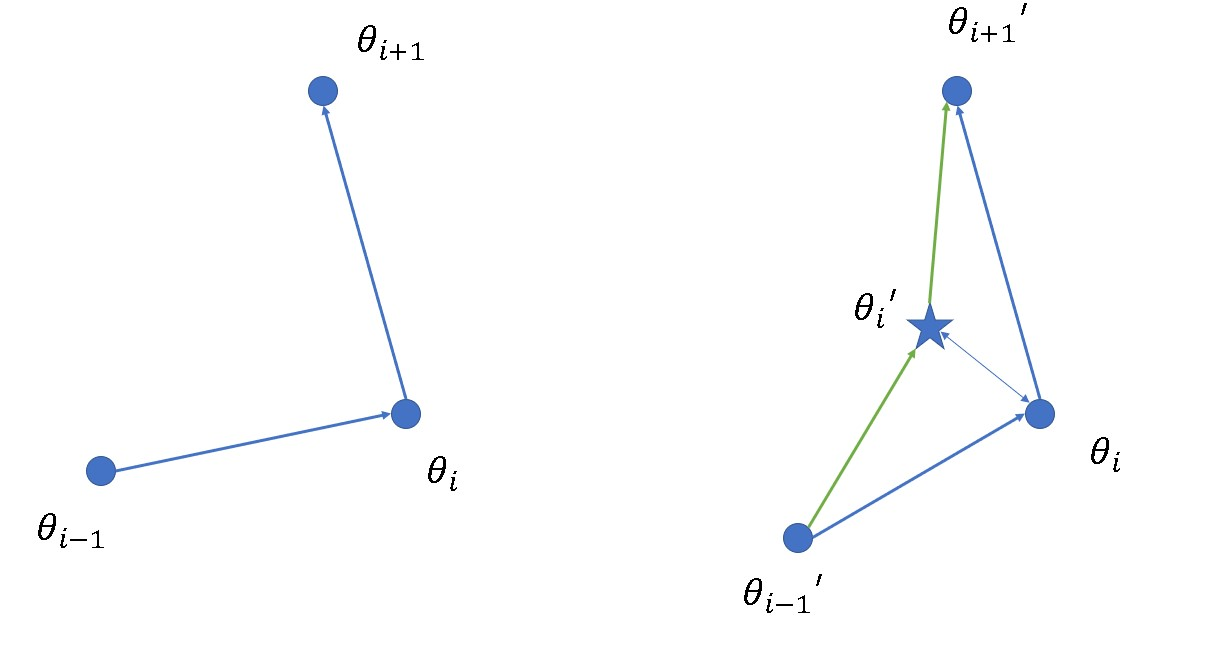
\includegraphics[width=0.5\hsize]{fig/5-conclusion/diagram.jpg}
\caption{The illustration of path smoothing algorithm}
\label{fig::conclusion::pathsmooth}
\end{figure}

\subsection*{実機の性能向上}
\secref{sec::result::consideration}で述べた通り,実機にはいくつかの課題が残っている.まずは,ハンドの取り付けについてである.前述の通り,現在のハンドは関節とリンク間に遊びがあり,またサーボモータにかかる負荷も大きい.前者について,3Dプリンタによるリンク作成は手軽であり,リンク自体も十分な精度で,かつ軽量にできる.しかし,耐久性は十分ではなくねじによる結合部が経年劣化する.そこで,耐久性に優れた軽量な素材を使用し,機械加工により固定する等の対策が必要である.後者については,\secref{sec::result::consideration}の通り,ボールキャスタによる解決策が考えられる.これにより,片持ち状態を解消でき,前者の劣化の問題も解消できるかもしれない.\par
また,リンク間に間隙が存在し,マニピュレーション中に対象物の角が入り込む場合があることも述べた.そのため,関節部に円板を取り付けることで間隙を消す必要がある.これに応じて,動作計画でリンクと円板を考慮した$C_{\mathrm {free\_obj}}$が算出されるように修正する必要がある.


% 白魔術
\expandafter\ifx\csname ifdraft\endcsname\relax
    \end{document}
\fi
